\documentclass[aspectratio=169, table]{beamer}

\usepackage[utf8]{inputenc}
\usepackage{listings} 

\usetheme{Pradita}

\subtitle{MTI104 - IT Services}

\title{Session-08:\\\LARGE{Practices to Enable Service \\Support}}
\date[Serial]{\scriptsize {PRU/SPMI/FR-BM-18/0222}}
\author[Pradita]{\small{\textbf{Alfa Yohannis}}}

\begin{document}

\frame{\titlepage}

\begin{frame}
\frametitle{Service Life Cycle}

A service is conceived, designed, built, and supported throughout its life cycle. Key aspects include:
\begin{itemize}
	\item Services are supported to ensure proper functioning.
	\item Break-fix is applied when issues occur.
	\item Smaller modifications are done ad hoc.
	\item Major changes undergo a continual improvement cycle.
	\item Activities visible to stakeholders highlight achievements.
	\item Enablers support service support practices.
	\item This chapter covers three support enabling practices.
\end{itemize}

\end{frame}

\begin{frame}
\frametitle{Support Enabling Practices}

The three support enabling practices discussed are:
\begin{itemize}
	\item Information Security Management
	\item IT Asset Management
	\item Service Configuration Management
\end{itemize}

\end{frame}

\begin{frame}
\frametitle{Information Security Management Overview}

Information Security Management is crucial due to increasing threats:
\begin{itemize}
	\item Introduced in design, not as an afterthought.
	\item Blurred lines with DevSecOps and Rugged DevOps.
	\item ITIL retains exclusivity in managing internal security.
	\item Collaboration with DevSecOps for external interfaces.
\end{itemize}

\end{frame}

\begin{frame}
\frametitle{Information Security Management Practice}

The purpose is to protect the organization's information:
\begin{itemize}
	\item Implement security controls, policies, and processes.
	\item Activities include Detection, Correction, Prevention.
	\item Detection: Monitoring and identifying threats.
	\item Correction: Addressing detected threats.
	\item Prevention: Avoiding future threats.
\end{itemize}

\end{frame}

\begin{frame}
\frametitle{Information Security Threats}

Key areas of information security threats include:
\begin{itemize}
	\item Confidentiality: Unauthorized access protection.
	\item Integrity: Prevention of unauthorized modifications.
	\item Availability: Ensuring access to authorized parties.
	\item Authentication: Identifying and verifying entities.
	\item Nonrepudiation: Proof of actions and agreements.
\end{itemize}

\end{frame}

\begin{frame}{Areas of information security}
	 \frametitle{ Areas of information security}
\begin{center}
	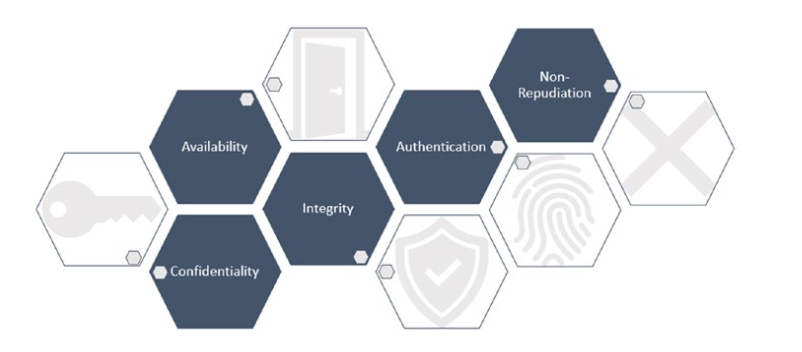
\includegraphics[width=0.7\linewidth]{images/image-01.png}
\end{center}
\end{frame}

\begin{frame}
\frametitle{Information Security Areas}

Expanding field of information security:
\begin{itemize}
	\item Confidentiality, Integrity, Availability.
	\item Added areas: Authentication, Nonrepudiation.
	\item Evolution from ITIL v3 to the current framework.
\end{itemize}

\end{frame}

\begin{frame}
\frametitle{Information Security in Service Value Chain}

Information Security Management in SVC:
\begin{itemize}
	\item Plan: High involvement.
	\item Design and Transition: High involvement.
	\item Obtain/Build: High involvement.
	\item Engage: High involvement.
	\item Deliver and Support: High involvement.
	\item Improve: High involvement.
\end{itemize}

\end{frame}

\begin{frame}
\frametitle{IT Asset Management Overview}

IT Asset Management involves:
\begin{itemize}
	\item Planning and managing IT asset life cycles.
	\item Maximizing value and controlling costs.
	\item Managing risks and supporting decision-making.
	\item Meeting regulatory and contractual requirements.
\end{itemize}

\end{frame}

\begin{frame}{Life cycle of an IT asset}
	 \frametitle{ Life cycle of an IT asset}
\begin{center}
	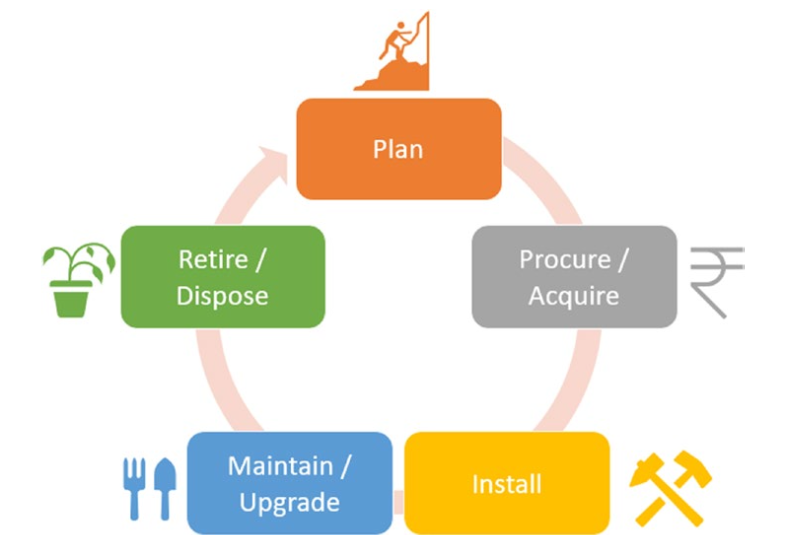
\includegraphics[width=0.5\linewidth]{images/image-02.png}
\end{center}
\end{frame}

\begin{frame}
\frametitle{IT Asset Management Practice}

Purpose and importance of IT asset management:
\begin{itemize}
	\item Tracking asset life cycles.
	\item Managing procurement, reuse, retirement, disposal.
	\item Reducing risks and controlling costs.
	\item Complying with standards and regulations.
\end{itemize}

\end{frame}

\begin{frame}
\frametitle{Types of Asset Management}

Types of asset management include:
\begin{itemize}
	\item Hardware Asset Management
	\item Software Asset Management
	\item Client Asset Management
	\item Cloud-Based Asset Management
\end{itemize}

\end{frame}

\begin{frame}
\frametitle{Service Configuration Management}

Importance of Service Configuration Management:
\begin{itemize}
	\item Manages configurations and components.
	\item Essential for complex systems with multiple dependencies.
	\item Foundation for project success and service delivery.
\end{itemize}

\end{frame}

\begin{frame}
	\frametitle{ITIL Definition of Service Configuration Management}
	\begin{itemize}
		\item Purpose: Ensure accurate and reliable configuration information
		\item Includes CIs and their relationships
		\item Provides a blueprint of IT services and dependencies
		\item Enables ease of change, impact analysis, and outage resolution
		\item Keeps configuration data alive and accessible
		\item Avoids problems from lack of configuration management
		\item Essential for current fast-changing environments
	\end{itemize}
\end{frame}

% Slide 2
\begin{frame}
	\frametitle{Configuration Items (CI)}
	\begin{itemize}
		\item CI: Component managed to deliver an IT service
		\item Examples: Servers, routers, applications
		\item Can be individual components or whole systems
		\item Decision on CI level: Configuration architect
		\item Attributes: Owner, location, status, etc.
		\item Controlled through change management
		\item Ensures accuracy and prevents unauthorized changes
	\end{itemize}
\end{frame}

\begin{frame}{Configuration management system (CMS)}
	 \frametitle{ Configuration management system (CMS)}
\begin{center}
	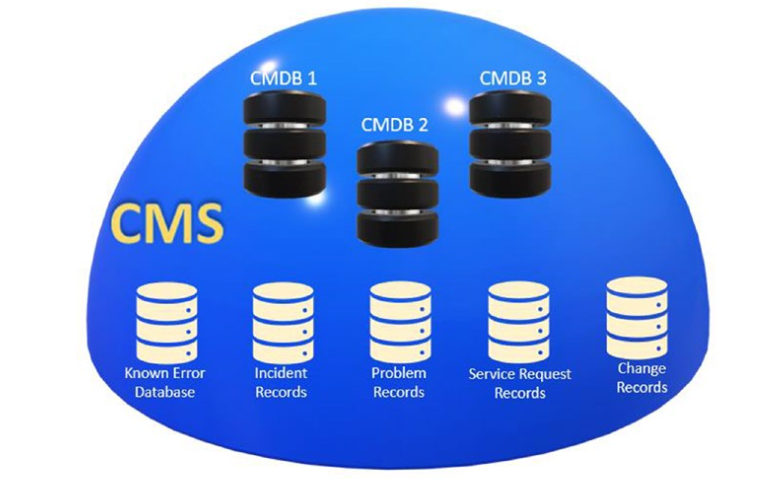
\includegraphics[width=0.6\linewidth]{images/image-03.png}
\end{center}
\end{frame}

% Slide 3
\begin{frame}
	\frametitle{CMDB, CMS, and Service Model}
	\begin{itemize}
		\item CMDB: Repository of CIs and their relationships
		\item Tracks dependencies and impacts visually
		\item CMS: Integrates multiple CMDBs and other databases
		\item Service Model: Graphical view of CMDB
		\item Shows relationships between interconnected CIs
		\item Assists in incident and change management
		\item Value in application, not just representation
	\end{itemize}
\end{frame}

\begin{frame}{Illustration of a service model}
	 \frametitle{ Illustration of a service model}
\begin{center}
	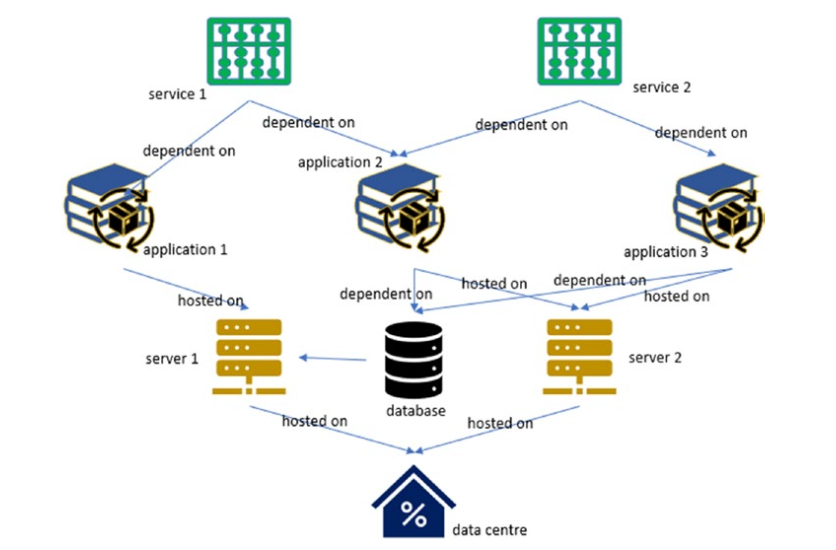
\includegraphics[width=0.5\linewidth]{images/image-04.png}
\end{center}
\end{frame}

% Slide 4
\begin{frame}
	\frametitle{Primary Activities of Service Configuration Management}
	\begin{itemize}
		\item Identify and populate CIs in CMDB
		\item Modify CMDB with changes
		\item Conduct periodic validations
		\item Use auditors and discovery tools for accuracy
		\item Validate CIs in CMDB and against physical CIs
		\item Ensure changes are authorized and accurate
		\item Maintain up-to-date configuration data
	\end{itemize}
\end{frame}

% Slide 5
\begin{frame}
	\frametitle{Engagement in Service Value Chain}
	\begin{itemize}
		\item Plan: Low involvement, but useful for change proposals
		\item Design and Transition: High involvement, supports design changes
		\item Obtain/Build: CIs created during this phase
		\item Engage: High involvement, identifies dependencies
		\item Deliver and Support: Leverages CIs for efficiency
		\item Improve: Medium involvement, adapts to improvements
		\item Evolving practice based on IT needs
	\end{itemize}
\end{frame}

\begin{frame}
	\frametitle{Multiple Choice Question}
	\textbf{Which of the following is the right definition of an IT asset?}
	\begin{itemize}
		\item[A.] An IT component that goes through the life cycle starting from procurement to disposal
		\item[B.] A component that has a financial value and is owned by the service provider to provide services
		\item[C.] An IT component that is required to deliver a service
		\item[D.] Any financially valuable component that can contribute to the delivery of an IT product or service
	\end{itemize}
\end{frame}


\end{document}
